\chapter{Lecture 12 - Supercritical CO$_{2}$ Brayton Cycles}
\label{ch:ch12}
\section{Objectives}
The objectives of this lecture are:
\begin{enumerate}
\item Illustrate the benefits of S-CO$_{2}$ Brayton cycles.
\item Show why regeneration is so important for S-CO$_{2}$ cycles.
\item Provide an alternative definition of regenerator effectiveness that one should use for supercritical gas power cycles.
\end{enumerate}

\section{CO$_{2}$ Brayton Cycles}

\newthought{When we introduced the Brayton cycle,} we used helium as the working fluid.  Indeed helium is a highly favored choice for numerous small modular reactor concept designs for high temperature reactors and we found that high cycle thermal efficiency could be obtained even with a simple (albeit ideal) Brayton cycle.  Helium, however, has some problems; some of these include:\cite{dostal2006supercritical}
\begin{itemize}
\item Helium is expensive.
\item Power conversion systems using helium can expect significant helium leakage through seals of rotating components and even welded boundaries.
\item Helium power cycle efficiency is more sensitive to regenerator effectiveness and fractional hydraulic pressure drops in plant components.
\item There is less experience World-wide in the use of Helium as a working fluid compared to air and CO$_{2}$.
\end{itemize}
For these reasons, for the time being, we will shift the focus of our attention to Brayton cycles using CO$_{2}$ as the working fluid.  

\newthought{Let us consider} a simple, ideal, closed Brayton cycle using CO$_{2}$ as the working fluid.  $P_{\text{max}}=2000$ kPa and $P_{\text{min}}=770$ kPa.  A schematic of the system and performance results are shown in Figure \ref{fig:co2_brayton_results}.

\begin{figure}
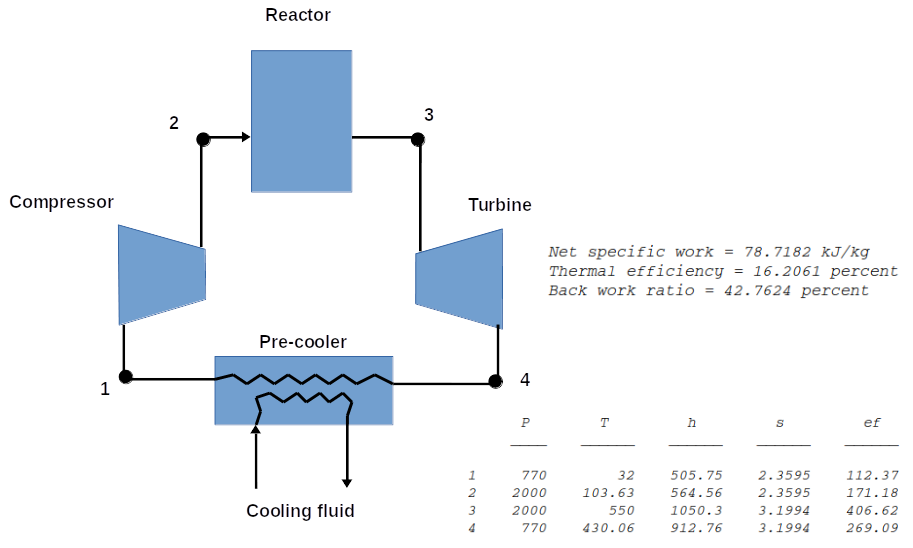
\includegraphics{co2_brayton_results.png}
\caption{Simple ideal Brayton cycle with CO$_{2}$}
\label{fig:co2_brayton_results}
\end{figure}

\newthought{From the state point table} it is evident that the fluid is still at a high temperature at the turbine exhaust; a considerable fraction of the energy/exergy provided by the reactor is rejected to the atmosphere. We can also see that the back work ratio is quite high. 

\subsection{Simple Supercritical CO$_{2}$ Brayton Cycle}

\begin{marginfigure}
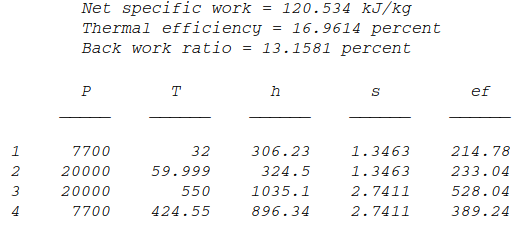
\includegraphics{sco2_brayton_results.png}
\caption{Analysis of simple Supercritical CO$_2$ Brayton Cycle}
\label{fig:sco2_brayton_results}
\end{marginfigure}

\newthought{Taking our lead} from the title of this lecture, we will examine how system performance changes when we increase system pressure above the critical pressure for CO$_{2}$ which is approximately 7.4 MPa while maintaining the same maximum temperature and pressure ratio.  The numerical results from the analysis are presented in Figure \ref{fig:sco2_brayton_results}. 

Note that the back work ratio has been drastically reduced. By pressurizing the CO$_2$ above the critical pressure, the specific volume is lower and the specific pump work has been reduced.  Still, the thermal efficiency is very low; we're still throwing away too much energy in the pre-cooler. A regenerator is definitely needed.

\subsection{Supercritical CO$_2$ Regenerative Brayton Cycle}
\newthought{We want to} reduce the amount of exergy rejected to the environment so we modify the cycle to add a regenerator.  We will choose a very optimistic regenerator effectiveness of 90\% while maintaining all other system parameters the same.\sidenote[][-0.5cm]{We will justify this optimisim by pointing to the expected heat transfer improvement with the CO$_{2}$ at high pressure and density.  We will also take comfort in the fact that the textbook assumes similar regenerator effectiveness for supercritical CO$_{2}$ cycles.}  A schematic of the cycle and analysis results are provided in Figure \ref{fig:sco2_brayton_regen_results1}
\begin{figure}
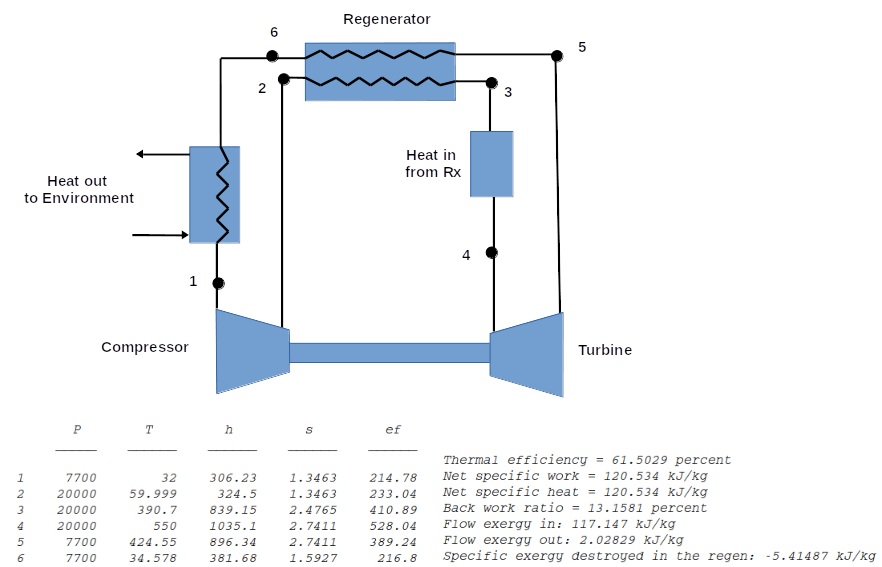
\includegraphics{sco2_brayton_regen_results1.png}
\caption[][1cm]{Regenerating S-CO$_{2}$ cycle.}
\label{fig:sco2_brayton_regen_results1}
\end{figure}

\newthought{As the results indicate,} adding regeneration did nothing to change net specific work, it's still at 120.5 kJ/kg, but recapturing that otherwise wasted energy, according to the analysis results in thermal efficiency increasing to over 61\%.(!!)  Before popping open the Champagne we should review the results of the exergy analysis.\sidenote{Before looking at the numbers repeat to yourself: ``\emph{Exergy} in minus \emph{exergy} out equals \emph{exergy} transfered through work plus \emph{exergy} destroyed.''} In round numbers, specific flow exergy passed in to the working fluid from the reactor is 117 kJ/kg, exergy rejected to the environment in the pre-cooler is a mere 2 kJ/kg; think of this as 115 kJ/kg of exergy being provided to the cycle for use.  But somehow we extracted 120 kJ/kg of specific work!?!  The explanation, and the sore thumb that should stick out at you when you examine the results, is the \underline{\emph{negative}} specific exergy destruction rate calculated for the regenerator.  What happened?

\newthought{The problem} is contained in our definition of regenerator effectiveness; not that it is necessarily too high, but that it is inadequate for this problem involving a fluid above its critical pressure.  Recalling from a previous lecture, we defined the regenerator effectiveness as:

\begin{equation}
\eta_{\text{reg}} = \frac{\Delta h_{\text{actual}}}{\Delta h_{\text{max}}} = \frac{h_3 - h_2}{h_5 - h_2}
\label{eq:regen_eff2}
\end{equation}   
but this formulation leaves out a key piece of physics: heat transfer, in a regenerator or elsewhere, is driven by temperature differences; the equation above only considers enthalpy values. Temperatures at the inlets and outlets of the regenerator for this analysis are shown in Figure \ref{fig:regen_temp_bad}. Note that the temperature at state point 6 (regenerator hot side outlet) is \underline{\emph{lower}} than state point 2 (cold side inlet).  This is obviously a violation of the 2nd law of thermodynamics.
\begin{marginfigure}
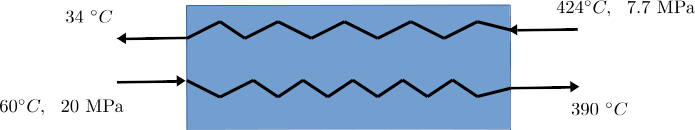
\includegraphics{regen_temps_bad.png}
\caption{Regenerator temperatures.}
\label{fig:regen_temp_bad}
\end{marginfigure}
We can re-connect enthalpy with temperature by using the specific heat at constant pressure, $C_p$.  Using this we can re-write Equation \ref{eq:regen_eff2} as:
\begin{equation}
\eta_{\text{reg}}=\frac{C_p(T_3 - T_2)}{C_p(T_5 - T_2)}
\label{eq:regen_eff3} 
\end{equation}

\begin{marginfigure}
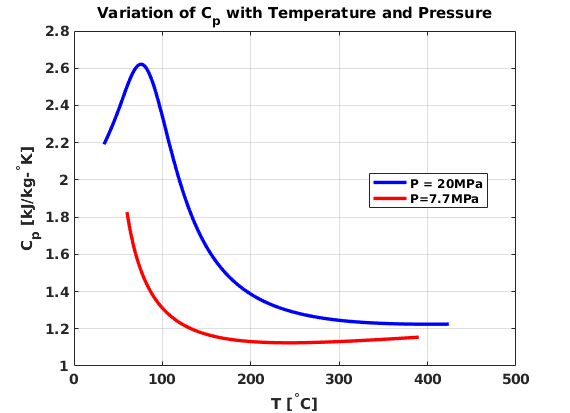
\includegraphics{variation_of_Cp_sco2_brayton_regen.png}
\caption{Variation of $C_p$ within the regenerator.}
\label{fig:cp_var}
\end{marginfigure}

This does not look like a great leap forward but we can now see that Equation \ref{eq:regen_eff3} leaves another detail out: the specific heat is \underline{not} constant.  A plot of specific heat at constant pressure for the high pressure and low pressure side of the regenerator is shown in Figure \ref{fig:cp_var}. 

An improvement can be made by refining our definition of regenerator effectiveness further\cite{bergman2011introduction} as follows:
\begin{equation}
\eta_{\text{reg}}=\frac{q}{q_{\text{max}}}=\frac{C_c(T_{c,o}-T_{c,i})}{C_\text{min}(T_{h,i}-T_{c,i})} = \frac{C_h(T_{h,i}-T_{h,o})}{C_\text{min}(T_{h,i}-T_{c,i})}
\label{eq:regen_eff4}
\end{equation}
where $C_c$ and $C_{\text{min}}$ refer to the specific heat at constant pressure for the cold stream and the minimum specific heat at constant pressure respectively.  But what is a good choice for either $C_c$ or $C_h$? ---they both change significantly over the temperature range of interest.
\begin{marginfigure}
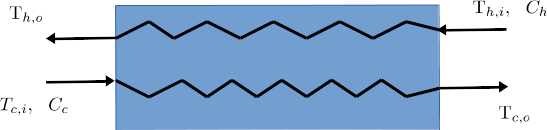
\includegraphics{regen_t_schm.png}
\caption{Regenerator schematic}
\label{fig:regen_t_schm}
\end{marginfigure}

\newthought{The method we will use} is based on techniques described in a technical report from MIT\cite{dostal2004supercritical} and is given in Equation \ref{eq:regen_eff_sc}.

\begin{equation}
\eta_{\text{reg}} = \frac{h_3 - h_2}{h_5 - h_{P_6,T_2}} = \frac{h_5 - h_6}{h_5 - h_{P_6,T_2}}
\label{eq:regen_eff_sc}
\end{equation}
where $h_{P_6,T_2}$ is the enthalpy evaluated at the pressure of state point 6 (low pressure outlet), but the temperature at state point 2 (low temperature inlet).  This ensures that the denominator of Equation \ref{eq:regen_eff_sc} represents a maximum enthalpy change. 
\subsection{Supercritical CO$_{2}$ Regenerative Cycle Revisited}
Using this new method the cycle will be re-analyzed with all of the same parameters as before.  The results are presented in Figure \ref{fig:sco2_brayton_regen_results2}.  Once again, as expected, there is no change to the net specific work.  For this analysis, the thermal efficiency is a respectable 37.7\% and there is no negative exergy destruction.
\begin{marginfigure}
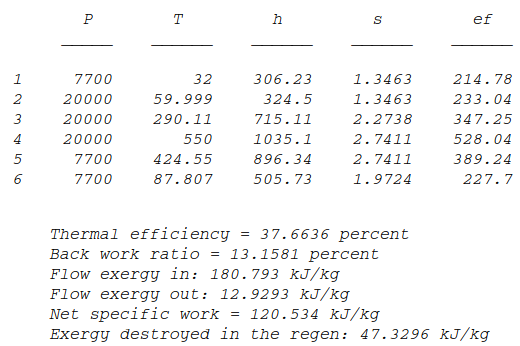
\includegraphics{sco2_brayton_regen_results2.png}
\caption{Regenerated S-CO$_{2}$ results with revised $\eta_{\text{reg}}$}
\label{fig:sco2_brayton_regen_results2}
\end{marginfigure}  
\newthought{You should note} the fairly high value of exergy destruction for the regenerator; particularly considering the optimistic regenerator effectiveness that we assumed.  Recall that exergy destruction is how we quantify irreversibility, and for heat transfer processes such as what occurs in the regenerator, irreversibility comes from transferring heat across temperature gradients.\sidenote[][-0.5cm]{Of course you need at least an infinitesimal temperature gradient to transfer heat; reversible heat transfer must take place across such an infinitesimal temperature gradient.} Plotting, as we did before, the temperatures at the inlets and outlets of the regenerator in Figure \ref{fig:regen_temps_good}, we get some idea as to the source of the extensive exergy destruction. Note the high differential temperature between the fluids at the right end of the regenerator as well as the significantly different change in temperature for the low- and high-pressure fluids respectively.
\begin{marginfigure}
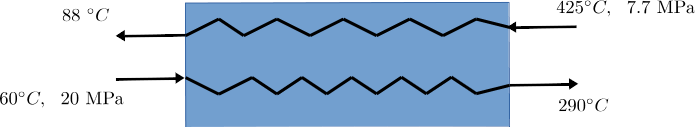
\includegraphics{regen_temps_good.png}
\caption{Regenerator temperatures with revised effectiveness.}
\label{fig:regen_temps_good}
\end{marginfigure}
\newthought{The variation in temperature} change can be better understood in light of the variation of $C_p$ as shown before in Figure \ref{fig:cp_var}. On the high-pressure side, especially at lower temperatures, $C_p$ is much higher than it is at high temperature and low-pressure side.  This means that, if we have the same mass flow rate of working fluid on both the low- and high-pressure side of the heat exchanger, we will not be able to avoid having large differences in the temperature change.

A resolution to this issue will be introduced in the next lecture.  We will break the regenerator up into two stages: a low temperature regenerator and a high temperature regenerator.  In the low temperature regenerator, where the variation in $C_p$ between the fluids is greatest, we will reduce the mass flow rate on the high-pressure/low-temperature side.  This will allow the temperature changes on each side of the regenerator to be better matched.  Overall this scheme will result in effective regeneration with reduced exergy destruction and correspondingly improved efficiency.

